\subsection{Objectives}
\label{sub:objectives}
\smallskip

The proposal’s overarching aim is to discover or constrain the particle nature of dark matter via its production at the LHC, 
in synergy with the broader DM experimental and theory community. 
The basis for reaching this aim is the implementation of data-taking techniques that enable the ATLAS experiment to obtain a much bigger physics output from the upcoming LHC dataset without requiring a significant increase in resources. 
Physics results and software tools resulting from this proposal will be shared, in line with Open Science and FAIR principles.
The objectives of each WP in this proposal are described in the following sections. 
%, while the impact and associated risks and mitigation strategies are described in Sec.~\ref{sec:RiskImpact}.  

% and their interconnections are displayed in \textbf{Fig.~\ref{fig:WPs}}. 

\subsubsection{Objectives of WP1: advancing real-time analysis in ATLAS}

The first objective of WP1 is to \textbf{deploy a comprensive TLA stream in ATLAS within the new multithreaded ATLAS HLT software}. %mentioned above?
In Run-3, this project will allow offline-quality photons, muons and electrons to be used for physics analysis, in addition to jets. 
The success of the jet prototype has been demonstrated in Run-2 within my StG. 
The use of a jet TLA allowed to lower the HLT jet threshold from 420 GeV in traditional analysis to 220 GeV in TLA, bringing orders-of-magnitude improvements in the number of recorded events. 
%Impact for photons
A TLA implementation of HLT photons will bring significant improvements to the sensitivity of the dijet+ISR DM mediator search. 
The HLT analyzes all photon and electron candidates that have a $p_{\rm{T}}$ above 30 GeV, 
while only single-photon events with a $p_{\rm{T}}$ above 150 GeV are retained in traditional analysis. 
%The work done and lessons learned in the case of trigger-level jets will be the stepping stone for adding photons to the TLA stream, 
%and doubling the signal acceptance for the dijet+ISR search. 
The implementation of electrons and muons in TLA will follow that of photons.
% but they will not be a priority for first data as the difference in thresholds between online and offline events is limited. 
While electron and muon TLAs can still bring significant improvement to e.g. dark photon searches below the Z peak~\cite{ToBeCited}, %CMSDimuon
the aim of this work is to gain experience in the reconstruction and calibration of physics objects with constrained computing resources. 
%Secondary impact for the entire collaboration

The second objective of WP1 is to \textbf{implement and reconstruct a data stream combining physics objects reconstructed at the trigger level and selected raw information in restricted regions of the detector}, through the combination of the TLA and Partial Event Building (PEB) techniques. 
Deployed for the first time in ATLAS in this proposal, this combination will maintain a sufficiently small data format with an amount of information equivalent to traditional techniques. 
It will be a necessary ingredient to enable searches in WP4, and can be used for the characterization of any excesses observed in TLA searches. 
%The overall outcome of this work will be a technical publication detailing the early Run-3 trigger.  
Preliminary estimates based on the Run-2 $B-$physics PEB %cite muon paper if available
place the size of TLA+PEB events to less than half of a standard event. \\
\indent
To remain advantageous, TLA and PEB must have the minimal possible footprint in terms of both storage and computing power. 
Joint work betwen WP1 and WP2-4 will ensure that these constraints are met with dedicated trigger selections and selections.   
The budget of this proposal also includes storage servers that will be used to store this data in 2023-2024. 

\begin{wrapfigure}{L}{0.3\textwidth} 
\begin{center}
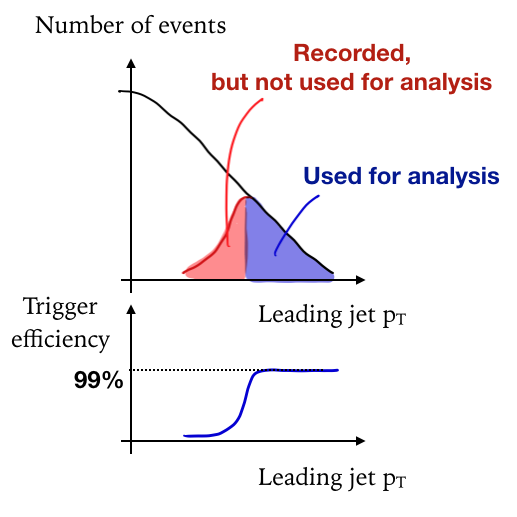
\includegraphics[width=0.28\textwidth]{figs_B2/efficiencySketch}
\caption{\color{black}\label{fig:wastedRate} \small Sketch of how trigger inefficiencies caused by a mismatch between the HLT and offline jet energy scales causes events to be recorded but never used for analysis.} %Trigger operation page
\end{center}
\vskip-5pt
\end{wrapfigure}

As a third objective of WP1, we will \textbf{develop the calibration techniques that are necessary to enable physics analysis} with a reduced HLT-level data format, achieving near-parity with offline performance. 
With my StG team, I have been responsible for reaching a 1-permille agreement between the jet energy scale of HLT jets with respect to offline jets in Run-2~\cite{ToBeCited}.%TLAPRL 
Within \textsc{Realdark} we will ensure that this is still the case for jets (as our main observables for WP3), as well as for other physics objects. 
%\color{red}\textbf{Not sure the following should be here, but it's a good motivation to calibrate HLT objects in case someone isn't convinced. }\color{black} 
Differences in the energy scale of HLT and offline objects also lead to inefficiencies in the trigger selection, as events that should pass the trigger are rejected due to HLT miscalibrations. 
As an example, the minimum $p_{\rm{T}}$ threshold applied to jets used in physics analysis is set to be higher than the HLT threshold due to these differences, leading to a substantial waste in terms of events that are recorded but not used for analysis, as shown in Fig.~\ref{fig:wastedRate}. 
Preliminary studies performed within my StG and with collaborators show that, due to the steeply falling jet energy spectrum, the amount of events that are recorded but never used by offline analysis can be as high as 60\% for certain trigger chains. 
The application of TLA-motivated improved calibration constants at the HLT during e.g. LHC technical stops (allowing sufficient time for the reoptimization of the trigger menu) will improve the fraction of useful data recorded and impact the overall ATLAS data taking strategies. 
%In WP1, my team and I will contribute to the simultaneous derivation of calibration constants for trigger and offline jets. 

The fourth objective of WP1 is to \textbf{further reduce the storage load of TLA events (and more generally ATLAS data and simulation) by compressing this data}. 
TLA data is ideally suited for studies of more aggressive (lossy) compression, since it has already been shown that is robust against reduced amounts of information using dedicated calibrations. If compression and decompression algorithms are sufficiently fast (order of milliseconds) they do not significantly increase the amount of resources needed for data processing. 
The use of machine learning techniques for fast and performant compression (e.g. of images) is widespread: inspired by this, my ATLAS collaborators and I have been supervising Lund University Master’s students in preliminary tests to compress TLA data using deep autoencoders~\cite{ToBeCited}. %cite autoencoders paper 
When compressing 2017 TLA jet data, these studies demonstrated that a compression of factor better than 2 can be achieved with a negligible performance loss.  
In this proposal we plan to continue this work and deploy this compression algorithm in a proof-of-principle yet realistic emulation of the trigger system using raw detector data. This is a future-looking study targeting HL-LHC, but if the results are ready to be deployed during the course of Run-3 we will use them for compression of the data recorded with techniques in WP1. 
%Is this also ok with TLA+PEB? 

As the trigger system is crucial for this research program and for the overall ATLAS physics output, the Lund group will maintain a leading role in its operations. 
Throughout the course of this project, the team members will be involved in the development and monitoring of trigger software. 
This is a particularly crucial responsibility during the run up to first data taking, after the complete overhaul of the ATLAS software. 
The Lund group has already taken responsibility roles in the trigger, with the StG postdoc William Kalderon (now a postdoctoral fellow at BNL), who has served for two years as the convenor of the jet trigger and has now moved on to be overall ATLAS trigger menu coordinator. 

\subsubsection{Objectives of WP2: commissioning the Run-3 trigger system with physics}

The overall objective of WP2 is the commissioning of the new trigger techniques using early LHC data, and their validation using well-established physics observables. 
These observables will be used to evaluate the performance of the calibration techniques and, if needed, implement corrective measures ahead of the production phase of LHC data taking. 

The first focus of WP2 is the \textbf{determination of the performance of HLT jets and photons, and of electrons and muons} at a later date. 
Together with our collaborators in ATLAS, we will evaluate the energy scale and the uncertainty of HLT objects using early data and simulation. 
I am an expert in those topics, having derived the very first iteration of the energy scale uncertainty~\cite{ToBeCited} %Jet cross-section and my thesis 
and having supervised a number of students on this topic since. 
Within my StG, we measured the performance of both offline and trigger jets in early Run-2 data using the same metrics and techniques, 
and we intend to do the same in Run-3 for an impact on all ATLAS early measurements and searches.  

We will use \textbf{early data to commission the new Run-3 trigger software} in the HLT dijet mass spectrum. 
The experience at the beginning of Run-2, where my collaborators and I observed a L1 trigger misconfiguration in early jet data that limited measurements and searches~\cite{Collaboration:2035503}, showed that this is a mandatory validation step to take after upgrades. 
Subsequently, we will repeat this process for PEB muons and electrons, using the dimuon and dielectron mass peaks from the decay of standard candles ($Z$ and $J/\psi$). 

\begin{wrapfigure}{R}{0.5\textwidth} 
\begin{center}
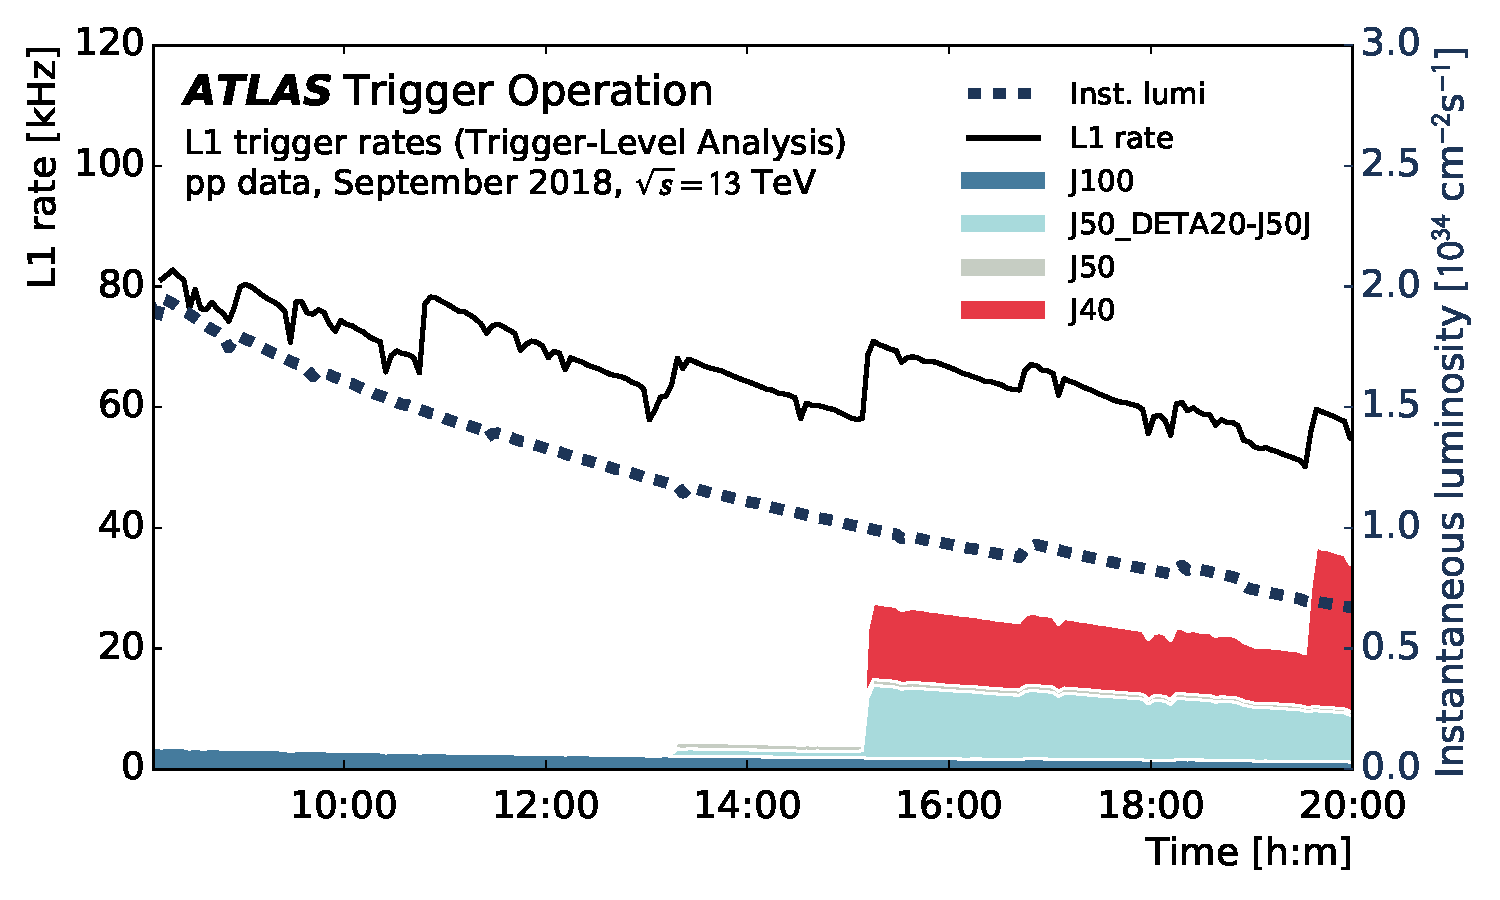
\includegraphics[width=0.48\textwidth]{figs_B2/TLAPublicWinter2019_L1Lumi.pdf}
\caption{\color{black}\label{fig:triggerLowThreshold} \small In Run-2, the underutilization of HLT resources at low LHC instantaneous luminosity allowed my team and collaborators to design TLA L1 triggers with reduced $p_\mathrm{T}$ thresholds~\cite{ToBeCited}.} %Trigger operation page
\vskip2pt
\end{center}
\end{wrapfigure}
%\vskip5pt

If the sensitivity of mediator searches in the dijet mass spectrum improves with respect to Run-2 results, we will publish dijet and dijet+ISR searches using early data.
As an example, if the LHC delivers more than $\approx$ 18/fb of low-luminosity runs, dijet searches can profit from much lower jet trigger thresholds as shown in Fig.~\ref{fig:triggerLowThreshold} and surpass sensitivity with respect to current searches\footnote{The analysis of the low-threshold Run-2 data is undergoing as part of my VR project grant, see Funding ID in Part B1}. 

Another important component of this proposal developed in WP2 is \textbf{reproducible end-to-end analysis software for dijet and dijet+ISR DM mediator searches}. 
We will use the RECAST framework to package the entire software stack used for early data analyses so that many of the steps can be executed automatically rather than manually.
Using RECAST at this early stage has three advantages. 
Firstly, it makes intermediate testing and monitoring much faster, as this code can be executed on new data and compared to already-tested data. 
Secondly, it shortens the time required to go from calibrated data to final plots and analysis results in the analysis iteration with the full LHC dataset in WP3.
Thirdly, it can be used as back-end to the REANA framework~\cite{ToBeCited}. %REANA
so that theorists and members of the DM community can test their own signals, as discussed in WP5.  

\subsubsection{Objectives of WP3: Dark matter mediator searches}

The overall objective of WP3 is to use Run-3 LHC data recorded with the TLA technique to search for new resonances in the dijet mass spectrum, motivated by DM mediators.
In this proposal we will focus on the decays of the mediators to light quarks, but the work in WP1 also enables dedicated searches for mediators decaying preferentially to heavy quarks. 

The main innovation in this WP is the \textbf{dijet+ISR photon search using the TLA technique}, alongside the gluon ISR signature. 
The two channels are complementary: the jet ISR channel is more sensitive due to higher signal rates, but selecting events using photon ISR can reach lower mediator masses. 
Both channels will be much more sensitive than current Run-2 traditional searches, since the threshold on the associated object is lowered from $\approx$ 400 GeV to $\approx$ 220 GeV and from $\approx$ 150 GeV to $\approx$ 40 GeV for jet and photon cases respectively.  
In turn, this increases the signal acceptance of more than one order of magnitude for a mediator mass of 250 GeV~\footnote{The background also increases, but since it is estimated using data-driven techniques as explained in~\ref{sec:methodologies} its increase can be managed without a significant loss in sensitivity.}, 
and it lowers the minimum mediator mass to which these searches are sensitive, as shown e.g. in Ref.~\ref{ToBeCited}.%CMS ISR TLA 
We will also maintain our involvement in the \textbf{full Run-2 + Run-3 dataset dijet TLA} towards a legacy TLA publication covering both LHC runs.

\subsubsection{Objectives of WP4: Dark sector searches}

%CD: I have the feeling this is a combination of objectives and methods
The objective of WP4 is to use Run-3 LHC data recorded with the TLA+PEB technique for dark QCD searches. 
The most promising parameter space to target will be determined by discussing the theory and broader DM community (WP5), and by using jet measurements to constrain dark QCD phenomenology. 
The rejection of QCD background at the HLT will be crucial for these searches, as it will allow recording higher signal rates in TLA+PEB events. 
The \textbf{search for semi-visible jets} will be performed first, adapting calibration and performance studies in WP1 and WP2 and analysis techniques in WP3 to this signature. 
Subsequently, we will augment the standard reconstruction techniques in WP2 to correctly identify anomalous content (e.g. leptons in jets) needed for the \textbf{composite jet search}.
An additional advantage of the PEB+TLA data stream selected for these searches is that it enables searches for a wide variety of non-standard jet topologies (e.g. photon-jets~\cite{ToBeCited}, %PhotonJets
jets containing long-lived particles~\cite{ToBeCited}) %Long lived jets
at a later date. 
This will have an impact especially after the end of this proposal when the long LHC shutdown is foreseen before HL-LHC and data already taken will be analyzed in further detail. 

\subsubsection{Objectives of WP5: Dissemination, communication, synergies}

The overall objective of WP5 is to connect the results in this proposal to the broader experimental community, with a focus on the search for DM, to maximize their impact. 
This WP naturally includes the contextualization, communication and dissemination of results, in terms of tools that can enhance the physics potential of experiments and of DM discoveries or constraints. WP5 covers my work within synergistic initiatives involving LHC experiments and the broader DM search communities that directly benefit the objectives of WP3 and WP4, started with the Dark Matter Forum and in the context of the update of the European Strategy of Particle Physics. Collectively furthering the DM community’s understanding of the theoretical and experimental landscape for WIMP and dark QCD models will sharpen the LHC search targets. WP5 spans the entire course of this project, and has four goals. 
\\
\indent
Firstly, we will collaborate with theory experts in Lund, Heidelberg, Aachen and worldwide to \textbf{identify the most promising parameter space for the searches in WP4}.
Concretely, this will take place through shared supervision of PhD students and dedicated workshops in Lund, similar to the 2019 Dark Jets workshop~\cite{ToBeCited}. %DarkDijetsWorkshop
These workshops will allow cross-talk with the community interested in comparing and contrasting regular and dark QCD, leading e.g. to concrete improvements for MC generation. 
\\
\indent
Secondly, I will \textbf{continue co-organizing the Initiative for DM in Europe and beyond (\href{https://indico.cern.ch/e/iDMEu/}{iDMEu})}, a cross-community effort focused on DM that includes the nuclear physics, astroparticle physics and particle physics communities. 
This initiative has more than 200 endorsers at the time of writing, and will have its first kick-off meeting in early Summer 2020. 
It has the ambition of becoming a permanent forum so that all different communities can identify opportunities to work together and exploit synergies and complementarities. 
Practical outcomes of work within this initiative are summary plots with commonly used benchmarks that enhance the complementarity of the LHC results in WP3 and WP4 with other experiments and astrophysical observations. iDMEu also includes a component of communication to the general public, also part of WP5. 
\\
\indent
Thirdly, we will \textbf{disseminate the technical outcomes of WP1 to other experiments at the LHC and beyond}. 
This will be achieved via technical peer-reviewed papers that include links to prototype open source software implementations as auxiliary materials and presentation in conferences. 
I have recently become part of the coordination team of the cross-experiment \href{https://hepsoftwarefoundation.org}{HEP Software Foundation} (HSF). 
With its goal of helping experiments meeting the challenges posed by new experimental programmes for HL-LHC, the HSF is an ideal platform to connect the solutions in this proposal to experimental needs. 
%This goal also includes concrete work on data compression with the EGO/Virgo experiment. 
\\
\indent
The fourth goal of WP5 is to \textbf{make results and data from WP3 and WP4 as accessible as possible}, both inside and outside the ATLAS collaboration. 
We will publish the final analysis likelihoods from WP2-4 and implement the end-to-end RECAST analyses in the REANA hub~\cite{ToBeCited}, %REANA
so that they can be scrutinized and reproduced without a need to directly access ATLAS data (which will only be available in open format at a later date).
These analyses will become part of a broader effort the cross-experiment \textit{Virtual DM environment} for end-to-end data analysis within the European Science Cluster of Astronomy and Particle Physics ESFRI research infrastructure (ESCAPE), which I will start leading at the beginning of 2020. 
All software implementations within this project will become part of the \href{https://projectescape.eu/services/escape-software-data-catalogue}{ESCAPE Software Catalogue}. 




